\documentclass[numbers=endperiod]{scrartcl}



%test

%\usepackage{fontspec}
%\setmainfont{Calibri}
\renewcommand{\familydefault}{\sfdefault}


\usepackage{geometry}
\geometry{
	a4paper,
	total={170mm,257mm},
	left=20mm,
	right=20mm,
	top=20mm,
	bottom=39mm
}

\usepackage{fancyhdr}
\usepackage{lastpage}
\usepackage{graphicx}
\usepackage{caption}

\usepackage[table]{xcolor}% http://ctan.org/pkg/xcolor
%\captionsetup{belowskip=1pt,aboveskip=0pt}


\graphicspath{ {./images/} }
\renewcommand{\figurename}{Figuur }
\renewcommand{\tablename}{Tabel }



\usepackage{xcolor}

\definecolor{hhs_theme_heading_1}{RGB}{26,104,169}
\definecolor{hhs_theme_heading_2}{RGB}{179,214,243}
\definecolor{hhs_theme_heading_3}{RGB}{170,183,52}

\addtokomafont{section}{\normalfont\Large}

\setkomafont{section}{\sectionheading}
\newcommand{\sectionheading}[1]{%
	\normalfont
	\Large%\sf\bf%
	\setlength{\fboxsep}{0cm}%already boxed
	\colorbox{hhs_theme_heading_1!80}{%
		\begin{minipage}{\linewidth}%
			\vspace*{6pt}%Space before
			\hspace*{4pt}
			\color{white}
			#1
			\vspace*{4pt}%Space after
		\end{minipage}%
}}

\setkomafont{subsection}{\subsectionheading}
\newcommand{\subsectionheading}[1]{%
	\normalfont
	\setlength{\fboxsep}{0cm}%already boxed
	\colorbox{hhs_theme_heading_2!80}{%
		\begin{minipage}{\linewidth}%
			\vspace*{4pt}%Space before
			\hspace*{2pt}
			#1
			\vspace*{2pt}%Space after
		\end{minipage}%
}}

\setkomafont{subsubsection}{\subsubsectionheading}
\newcommand{\subsubsectionheading}[1]{%
	\normalfont
	\noindent
	
		\begin{minipage}{\linewidth}%
			\textcolor{hhs_theme_heading_1}{\rule{\textwidth}{1.5pt}}
			\vspace*{4pt}%Space before
			\hspace*{-29pt}
			#1
			\vspace*{2pt}%Space after
		\end{minipage}%
}
%end test



\DeclareGraphicsExtensions{.pdf,.png,.jpg}
\pagestyle{fancy}
%\fancyhf{}
%\rfoot{Pagina \thepage \hspace{1pt} van \pageref{LastPage}}

\setlength{\headheight}{35pt} 
\setlength{\footheight}{135pt} 


\fancyhead[L]{%\begin{minipage}[b]{0.65\linewidth}
	
\includegraphics[scale=0.4]{Logo.png}
\fancyhead[C]{\vspace{-40pt}\textcolor{hhs_theme_heading_1}{\tiny In opdracht van: \\}
\includegraphics[scale=0.14]{rijkswaterstaat.jpg}}}
\fancyhead[R]{\slshape \leftmark}

\fancyfoot[L]{ 
\tiny 2016-11-22\textunderscore PVA\textunderscore Ricardo-Molenaar\\\textunderscore Martijn-van-Essen\textunderscore Plan-van-Aanpak\textunderscore vA01
}
\fancyfoot[C]{	%\begin{flushleft}
				%\hspace{100pt}
				%\vspace*{0pt}
				\small Ricardo Molenaar \& Martijn van Essen\\
				PROENT\\
				V1.0 \textbar 18-11-2016
				%\end{flushleft}
			}	
\fancyfoot[R]{\vspace{0pt}\small \textbar Pagina \thepage \hspace{1pt} van \pageref{LastPage}\textbar}


\renewcommand{\footrulewidth}{0.4pt}%

\title{My first document}
\date{18-11-2016}
\author{Martijn van Essen}

\usepackage{pdfpages}

\begin{document}
	%Title page
	\pagenumbering{gobble} %Turn off page numbers
	%\maketitle
	%\newgeometry{left=0cm,bottom=0cm}
	%\pagestyle{empty}
	%\vspace*{-3cm}
	%\includegraphics[scale=1]{cover.png}
	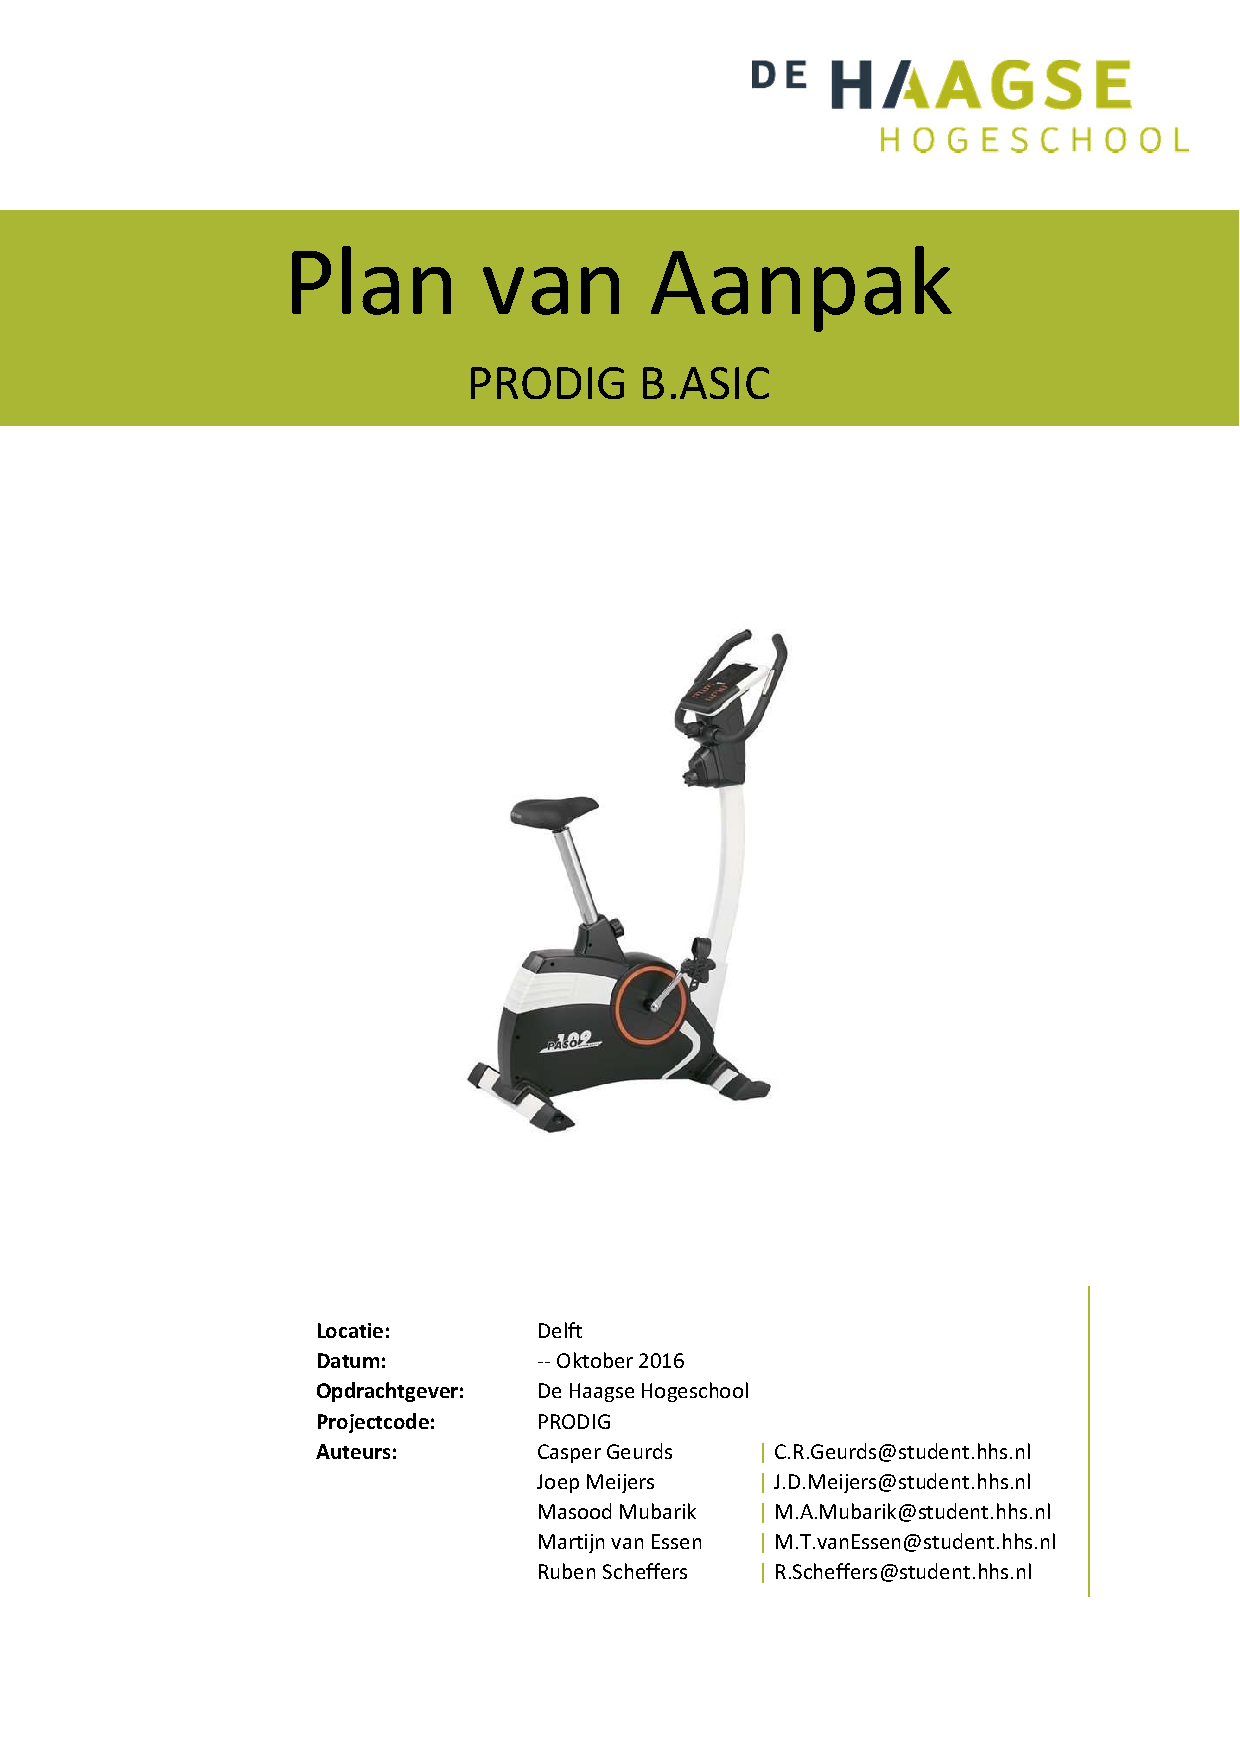
\includepdf{input}
	\newpage
	%\restoregeometry
	%End of title page
	
	%Versions page
	\pagenumbering{arabic} %Turn on page numbers
	\setcounter{secnumdepth}{0} %Turn off section numbering
	\section{Versiebeheer}
	
	\begin{center}
		\begin{tabular}{| p{4cm} | l | p{7cm} | l |}
			\hline
			
			\multicolumn{4}{|c|}{
				\cellcolor{hhs_theme_heading_2}
				Versiehistorie
			}  \\ \hline
			
			Versie 	& Datum 		& Wijzigingen 	& Auteur \\ \hline
			vA01 	& 22-11-2016 	& Alle wijzigingen 
			&Auteurs\\ \hline
		\end{tabular}
	\end{center}
	\newpage
	%End of Versions Page
	
	%Table of contents
	\renewcommand{\contentsname}{Inhoudsopgave} %Set table of contents section name
	\tableofcontents
	\newpage
	%End of Table of contents
	
	\setcounter{secnumdepth}{3}%Turn on section numbering

	\section{Projectachtergrond}
	Test
	\newpage

	\section{Projectresultaat}
	\newpage

	\section{Projectactiviteiten}
	\newpage

	\section{Projectgrenzen}
	\newpage

	\section{Kwaliteit}
	\newpage

	\section{Projectorganisatie}
	Het gestelde project is aangenomen door ingenieursbureau Molenaar \& van Essen. Dit bedrijf bestaat uit
	twee werknemers welke beide aan dit project zullen werken. 
	\begin{table}[h]
	\caption{Projectorganisatie}\label{table:Projectorganisatie}
	
		\centering
		\begin{tabular}{ p{.3\textwidth} | p{.32\textwidth} | p{.3\textwidth} }
			Naam: 				& Studentnummer:& E-mailadres \\ \hline
			Ricardo Molenaar 	& 15087506	 	& R.Molenaar@student.hhs.nl \\
			Martijn van Essen 	& 15086135		& M.T.vanEssen@student.hhs.nl \\
		\end{tabular}
	
	\end{table}
		\newpage

	\section{Planning}
	In tabel~\ref{table:Planning} is een planning voor het verloop van dit project weergegeven.
	\begin{table}[h]
	\caption{Projectplanning}\label{table:Planning}
	\centering
	\begin{tabular}{| p{.3\textwidth} | p{.32\textwidth} | p{.3\textwidth} |}
			\hline \rowcolor{hhs_theme_heading_2}
			Item: 				& Geschat begin:& Deadline \\ \hline
			Plan van Aanpak 	& 17-11-2016 	& 28-11-2016 \\ \hline
			Projectplan		 	& 28-11-2016	& 16-1-2017 \\ \hline
			Procesverslag(?)	& 9-1-2017		& 16-1-2017 \\ \hline
			Eindassessment		& 17-1-2017		& 24-1-2017 \\ \hline
		\end{tabular}
	\end{table}
	
	\newpage


	
%	\begin{equation}
%	f(x) = x^2
%	\end{equation}
	
\end{document}
